\documentclass[a4paper]{article}
\usepackage{amsmath}
\usepackage{amsfonts}
\usepackage{amssymb}
\usepackage{amsthm}
\usepackage{bm}
\usepackage{pdfpages}
\usepackage{caption}
\usepackage{graphicx}
\usepackage{multicol}
\usepackage{tabu}
\usepackage{thmtools}
\usepackage{verbatim}

% Page geometry
\usepackage{geometry}
\geometry{verbose,tmargin=2.4cm,bmargin=2.4cm,lmargin=2.4cm,rmargin=2.4cm}
\setlength{\columnsep}{0.8cm}

% Theorem formatting
\declaretheorem[style=definition,qed=$\blacksquare$,numberwithin=section]{Definition}
\declaretheorem[style=definition,qed=$\blacksquare$,numberwithin=subsection]{Prop}
\declaretheorem[style=definition,qed=$\square$,numberwithin=section]{Theorem}
\declaretheorem[style=definition,qed=$\square$,numberwithin=subsection]{Proof}
\declaretheorem[style=definition,qed=$\spadesuit$,numberwithin=section]{Procedure}
\declaretheorem[style=definition,qed=$\square$,numberwithin=section]{Corollary}
\declaretheorem[style=definition,qed=$\clubsuit$,numberwithin=section]{Result}

% Removes section numbering but continues counting
\renewcommand{\thesection}{}
\renewcommand{\thesubsection}{\arabic{section}.\arabic{subsection}}
\makeatletter
\def\@seccntformat#1{\csname #1ignore\expandafter\endcsname\csname the#1\endcsname\quad}
\let\sectionignore\@gobbletwo
\let\latex@numberline\numberline
\def\numberline#1{\if\relax#1\relax\else\latex@numberline{#1}\fi}
\makeatother

% New commands
\newcommand{\cas}{\stackrel{as}{\longrightarrow}}
\newcommand{\cid}{\stackrel{d}{\longrightarrow}}
\newcommand{\cip}{\stackrel{p}{\longrightarrow}}
\newcommand{\cov}{\text{Cov}}
\newcommand{\diag}{\text{diag}}
\newcommand{\ecdf}{\mathbb{F}_{n}}
\newcommand{\iid}{\stackrel{\text{IID}}{\sim}}
\newcommand{\plim}{\underset{n\to\infty}{\text{plim}}}
\newcommand{\seteq}{\stackrel{\text{Set}}{=}} 
\newcommand{\var}{\text{Var}}
\newcommand{\adj}{\text{adj}}

% Figure in multicol
\newenvironment{Figure}
  {\par\medskip\noindent\minipage{\linewidth}}
  {\endminipage\par\medskip}

% Page formatting
\usepackage{fancyhdr}
\pagestyle{fancy}
\lhead{MIT 6.867}
\rhead{Final Project}
\title{Developing Classifiers to Distinguish between Hepatocellular Carcinoma and Chronic Liver Disease based on Circulating Cell RNA-Seq Profiles}
\author{Divy Kangeyan, Zack McCaw, Kelly Mosesso}
\linespread{1.2}

\begin{document}
%%%%%%%%%%%%%%%%%%%%%%%
\maketitle

\begin{abstract}
Hepatocelluar carcinoma (HCC) is a major cause of morbidity and mortality in the developing world, and remains a significant disease burden in developed nations. The ability to identify HCC patients from amongst those with chronic liver disease (CLD) using a simple blood test would reduce treatment costs and facilitate early intervention. The circulating tumor cell (CTC) chip technology allows for efficient extraction of malignant cells and leukocytes from blood. Subsequent RNA-sequencing (RNA-seq) provides genome-wide RNA transcript profiles, which should enable accurate classification of subjects into disease categories. Here we aim to develop a model for HCC detection based on transcription profiles ascertained from circulating cells. We compare the classification performance of three prediction methods trained on each of three feature sets. Transcriptional features were selected by logistic regression, lasso, and random forests. Disease status was predicted by means of neural networks, support vector machines, and random forests. Model parameters were tuned by means of 20-times repeated 10-fold cross validation. Only two of the nine models outperformed the naive strategy of simply predicting that each testing observation belongs to the most common training data class. These were random forests and neural networks, each trained on features selected by lasso. We discuss the performance of each prediction strategy across feature sets, and within each feature set compare the performance of the different prediction strategies. 
\end{abstract}

\section{Introduction}

	Hepatocellular carcinoma (HCC) is the most prevalent subtype of liver cancer, and the third leading cause of cancer deaths. Worldwide, more than $5 \times 10^{5}$ patients are affected by HCC. Chronic liver disease (CLD), often instigated by hepatitis, is the major predisposing risk factor. The primary pathogenic pathway is thought to be infection and transformation of hepatic stem cells by the hepatitis B/C virus. If HCC is detected prior to metastasis, treatment by resection, radiation, or chemo-therapy can slow progression, and complete cure is possible by means of liver transplantation. 
	
	The Circulating Tumor Cell Center at Massachusetts General Hospital have developed the CTC-chip technology to remove erythrocytes and thrombocytes from whole blood, leaving samples enriched for (nucleated) leukocytes and circulating tumor cells, if present. The resulting sample contains gene expression signatures diagnostic of the component circulating tumor cells (CTCs) in cancer patients. Through contacts within this group at MGH, we have obtained expression data from RNA-seq analysis of both patients with CLD and HCC. The data set contains measurements for $\sim 59 \times 10^{3}$ transcripts for 84 patients -- 51 with HCC and 33 with CLD. 
	
	In excess of $80\%$ of HCCs occur in patients with preexisting cirrhosis, a gradual replacement of functional liver parenchyma by fibrotic scar tissue. The current standard of care for patients with cirrhosis is close clinical monitoring combined with MRI for diagnosis. However, the standard practice is resource intensive and beyond the scope of health care providers in low-resource settings where MRI machines are inaccessible. Thus, the ability to distinguish between patients with CLD and those with HCC based on expression analysis of a transportable blood sample (RNA-seq following CTC-chip) would represent a major clinical advance. Not only would this screening procedure accelerate detection and facilitate earlier intervention, it would reduce the cost of diagnosis and hopefully extend monitoring to low-resource settings \cite{davis2008hepatocellular}.
	
\section{Methods}
\subsection{Data preprocessing}
High throughput sequencing data contains both technical and biological variabilities. The main goal of sequencing studies is to understand the biological variabilities across samples; hence, there is a need to minimize the technical variabilities and other biases as much as possible. Since our data is count data from RNA-Seq technology we also performed some preprocessing methods before analyzing the data. First we removed any transcript that had zero variance across the samples, i.e. transcripts that had the same value for all patients. We also log transformed the counts to control extreme values in the transcript that could have occurred due to PCR amplification bias. Finally, we performed quantile normalization for the data. Quantile normalization is a widely used technique applied to high throughput sequencing data and microarray data \cite{bolstad2003comparison} \cite{hicks2015quantro}. Quantile normalization is performed to reduce technical variabilities in noisy datasets. In order to perform quantile normalization, the average of each quantile across samples is calculated, and this is used as the reference or the target. Then the values in the observed distribution are replaced with those from reference distribution for each sample, thereby forcing the observed and the reference distributions to be the same.


\subsection{Feature Selection}
\begin{figure}[h!]
	\centering
	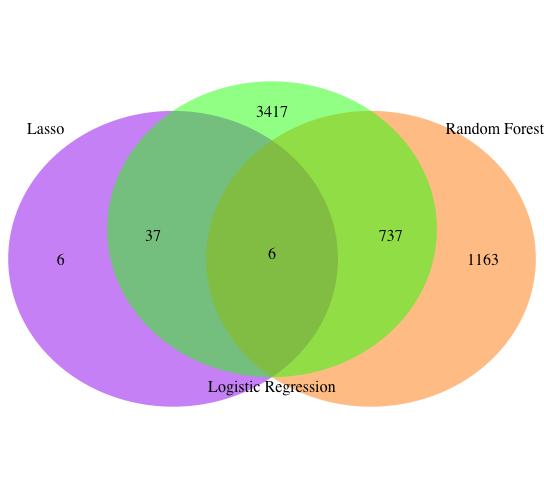
\includegraphics[scale=0.40]{venn.png}
	\caption{Venn diagram depicting the overlap between feature sets selected by lasso, random forests, and univariable logistic regression.}
	\label{fig:venn}
\end{figure}

\subsubsection{Feature Selection by Logistic Regression}
Logistic regression is type of generalized linear model (GLM) in which, conditional on the predictors, the outcome follows a Bernoulli distribution. In particular, suppose $y_{i}\in\{0,1\}$ is a binary outcome, $\bm{x}_{i}\in\mathbb{R}^{p}$ is a predictor, and that $y_{i}|\bm{x}_{i} \sim \text{Bern}[h(\bm{x}_{i}'\bm{\beta})]$. In GLM, the conditional expectation $E[y_{i}|\bm{x}_{i}]$ is modeled as a function $h(\cdot)$ of the linear predictor $\eta_{i} = \bm{x}_{i}'\bm{\beta}$. Here $\bm{\beta}$ is a vector of regression coefficients and $h : \mathbb{R} \to \text{dom}(E[Y|\bm{X}])$ is a mapping from $\mathbb{R}$ to the domain of the conditional expectation. In logistic regression, $h$ is taken as the sigmoid function $h(t) = (1+e^{-t})^{-1}$. Regression coefficients are estimated by means of maximum likelihood. In particular:
\begin{equation}
\bm{\hat{\beta}}^{\text{mle}} = \arg\max_{\bm{\beta}}\sum_{i=1}^{n}y_{i}\ln\big[ h(\bm{x}_{i}'\bm{\beta}) \big] + (1-y_{i})\ln\big[1-h(\bm{x}_{i}'\bm{\beta})\big]
\end{equation}
Given an estimate $\bm{\hat{\beta}}^{\text{mle}}$ of the regression coefficients, and an estimate $\hat{\text{se}}\big(\bm{\hat{\beta}}^{\text{mle}}\big)$ of the standard error (obtained from the inverse Fisher information matrix $\bm{\mathcal{I}}$) it is possible to assess the null hypothesis that the predictors are unassociated with the outcome, $H_{0}:\bm{\beta}=0$, using a Wald statistic. Rejection of this null hypothesis is of interest since transcripts that are not associated with the probability of having HCC are unlikely to have predictive utility. For our study, let $j$ index the $n_{g} = 49,128$ transcripts remaining after eliminating those with zero variance across samples, and let $a_{ij}$ denote the abundance of transcript $j$ in subject $i$. We fit $j=1,\cdots,n_{g}$ logistic regressions of the from $y_{i} = h(\bm{x}_{ij}'\bm{\beta}_{j})$ where $\bm{x}_{ij} = (1,a_{ij})'$ is the predictor and $\bm{\beta} = (\beta_{j,0},\beta_{j,1})'$ is the regression coefficient. Let $\hat{\beta}_{j,1}^{\text{mle}}$ denote the maximum likelihood estimate of the effect of transcript $j$ on the outcome. We calculate a $p$-value $\hat{p}\big(\hat{\beta}_{j,1}\big)$ via the Wald statistic which represents the probability of observe a coefficient estimate as far or further from zero than $\hat{\beta}_{j,1}^{\text{mle}}$ under the null hypothesis that $\beta_{j,1}$ is in fact zero. If $\hat{\beta}_{j,1}^{\text{mle}}$ is $\leq 0.05$ we reject $H_{0}$, and include transcript $j$ in the feature set. By design, this procedure has a false positive rate (i.e. type I error) of $5\%$ under the null, hence some transcripts selected into the feature set will only associate with disease status by chance.
Overall, $p = 4197$ features by marginal logistic regressions. 

\subsubsection{Feature Selection by LASSO}
% Synopsis of lasso
Lasso (least absolute shrinkage and selection operator) is a form of regression penalization that allows for simultaneous feature selection and coefficient estimation. Consider the linear regression model $\bm{y} = \bm{X}\bm{\beta} + \bm{\epsilon}$, where $\bm{y}$ is the outcome, $\bm{X}$ is the subject by feature design matrix, and $\bm{\epsilon}$ is a stochastic residual with mean zero and finite variance. The lasso estimator of the regression coefficients $\bm{\beta}$ is given by:
\begin{equation}
\bm{\hat{\beta}} = \arg\min_{\bm{\beta}}\big(\bm{y}-\bm{X}\bm{\beta}\big)'\big(\bm{y}-\bm{X}\bm{\beta}\big) + \lambda ||\bm{\beta}||_{1}
\end{equation} 
Here $\lambda$ is an adjustable tuning parameter. As $\lambda$ increases, the objective function is more heavily penalized for regression coefficients that are large in magnitude. Lasso's ability to perform feature selection derives from application of the non-smooth $\mathcal{L}_{1}$ norm to $\bm{\beta}$ in the lasso objective. It can be shown that lasso performs \textit{soft-thresholding} on the components of $\bm{\beta}$. Suppose $\bm{X}$ is orthogonal, either by design or via transformation (e.g. by principal component transform). Let $\hat{\beta}_{j}^{\text{ols}}$ denote the $j$th component of the ordinary least squares (OLS) estimate of $\bm{\beta}$. Now $\hat{\beta}_{j}^{\text{lasso}} = \text{sign}[\hat{\beta}_{j}^{\text{ols}}]\max\big(0,|\hat{\beta}_{j}^{\text{ols}}|-\lambda\big)$, i.e. lasso with tuning parameter $\lambda$ shifts the OLS estimates towards zero by a constant amount $\lambda$, and sets the coefficient exactly to zero if the shift would result in a change of sign. 

% Use of lasso for feature selection
For our study the outcome $y_{i}$ was binary, so feature selection was performed by lasso penalized logistic regression. The lasso estimates of regression coefficients are given by:
\begin{equation}
\bm{\hat{\beta}}_{\lambda}^{\text{lasso}} = \arg\min_{\bm{\beta}} -\ell(\bm{\beta}) + \lambda ||\bm{\beta}||_{1},
\end{equation}
where $h(t) $ and $\ell(\bm{\beta})$ are the same function described in the previous section. We estimated $\bm{\hat{\beta}}_{\lambda}^{\text{lasso}}$ on a grid of $10^{2}$ $\lambda$ values between $1/400$ and $1/4$, using the default settings of the \texttt{glmnet} function in \texttt{R}. Selection of a feature into the model corresponds to estimation of a non-zero regression coefficient using lasso. As $\lambda$ increases, only features with substantial predictive power provide a great enough increase in model (log) likelihood to offset the penalty on the magnitude of the regression coefficient. Consequently, as $\lambda$ increases, more features are forced out of the model. Since our training data consisted of $n=63$ observations, lasso could not select more than $p=63$ features, as adding additional features would lead to a model that was unidentified. We chose to set $\lambda$ to the minimum value considered by \texttt{glmnet}, since our goal at this stage was only to select features for subsequent model building, rather than to simultaneously develop a classifier. Overall, lasso selected $p=49$ features for use in model training. 

\subsubsection{Feature Selection through Random Forest Regression}
Random forest is an ensemble method based on decision trees. Decision trees have many appealing qualities including high interpretability and relatively low bias when they are grown deeply. However decision trees tend to have high variance in their prediction. Hence random forest utilizes the bagging technique where only fraction of the data is chosen to build large number of decision trees. These ensemble of trees are used to build a classifier and make predictions for new values. Since trees built by bagging are identically distributed they will have the same bias as an individual tree and averaging across those trees lower the variance. Therefore random forest benefits from low-bias decision trees and the bagging procedure that reduces the variance. \cite{friedman2001elements}

Random forest had high success rate in various settings in both classification and regression. The exact procedure for classification method will be explained in the prediction approaches section since we used random forest method for both feature selection and prediction. Although random forest method doesn't have the same level of interpretability as the decision trees, variable importance is a metric used to interpret the significance of a variable in a classification or regression setting and for feature selection. Variable importance can be calculated in several different ways, here we will explain two of the metrics to calculate the importance of a variable: Gini index and out of bag (OOB) sample error. 

Gini index is a measure of impurity. Gini index is specifically used in the classification setting and it is defined according to the equation shown below.

$$Q_m(T) = \sum_{k} \hat{P}_{mk}(1-\hat{P}_{mk})$$ 

where $ \hat{P}_{mk}$ is the probability of a sample from class k being split in $m^{th}$ split. Higher Gini index indicates less reliable split and lower Gini index shows a highly reliable split. In order to use this as a measure for feature selection, decrease in Gini produced by variable $j$ is calculated. In order to calculate the decrease in Gini, first the Gini index for the parent node is calculated then Gini index for the children nodes are calculated then difference in Gini index between the parent node and children nodes are calculated. This decrease in Gini is averaged across all the trees where the variable was utilized to produce the mean decrease in Gini. Variable that leads to the largest mean decrease in Gini is considered the one with the highest importance.

OOB sample error is calculated with the samples that are left out in the bagging procedure. When the $i^{th}$ tree is built, out of bag samples 
are used to calculate the prediction accuracy of the tree and then the value for the $j^{th}$ variable is randomly permuted in the out of bag samples and the accuracy is calculated again. The change in accuracy is calculated for all the trees for specific variable $j$ and averaged across them. Through this procedure mean change in the OOB sample error for $j^{th}$ variable is calculated. The variables that leads to large decrease in the OOB sample error are considered to have the highest importance. 

As mentioned earlier our data set had around 59000 features, however around 50000 of them did not decrease the Gini index in eventual split. Hence we selected top $3\%$ of the features based on the distribution of the mean decrease in the Gini index. Ultimately we selected 1906 features through random forest feature selection.


\subsection{Prediction Approaches}

\subsubsection{Prediction by Neural Networks}

Neural networks (NN) provide a flexible model for non-linear mapping of inputs to outputs. In contrast to GLMs where the relation between inputs and outputs is specified \textit{a prior}, NNs `learn' the mapping from the data. A neural network consists of an input layer, and output layer, and one or more hidden layers, where each layer is comprised of \textit{neurons} or computational units. The input layer is simply the set of predictors, in our case one for each transcript and an intercept. The hidden layers receive input from all units in the preceding layer, form a linear combination, then apply an activation function to the result. The output layer receives input for all units in the penultimate, hidden layer, form a linear combination, then apply an output function to generate a prediction. Suppose  $\bm{y}_{i} = (y_{i1},\cdots,y_{iq})'$ is continuous or categorical outcome of dimension $q$, and $\bm{x}_{i}\in\mathbb{R}^{p}$ is a predictor. A complete mathematical formulation of a neural network with one hidden layer of dimension $m$ takes the form:
\begin{gather}
\alpha_{ij}^{(1)} =\bm{x}_{i\bullet}'\Big(\bm{\omega}_{\bullet j}^{(1)}\Big),\;\; j = 1,\cdots,m \\
\bm{z}_{i\bullet}^{(1)} = \big(g_{1}(\alpha_{i1}^{(1)}),\cdots,g_{m}(\alpha_{im}^{(1)})\big)' \\
\alpha_{ik}^{(2)} = \Big(\bm{z}_{i \bullet}^{(1)}\Big)'\bm{\omega}_{\bullet k}^{(2)},\;\; k = 1,\cdots,q \\
\bm{\hat y}_{i} = \big(h_{1}(\alpha_{i1}^{(2)}),\cdots,h_{q}(\alpha_{iq}^{(2)})\big)'
\end{gather}
Here $\bm{\omega}_{\bullet j}^{(1)}$ is a $p$ dimensional weight vector, $\alpha_{ij}^{(1)}$ is the scalar linear predictor of unit $j$ in hidden layer 1, $g_{j}(\cdot)$ is an activation function, $\bm{\omega}_{\bullet k}^{(2)}$ is a $q$ dimensional weight vector, $\alpha_{ik}^{(2)}$ is the scalar linear predictor of unit $k$ in the output layer, $h_{k}(\cdot)$ is an output function, and $\bm{\hat{y}}_{i}$ is the predicted outcome. 

We considered a particular neural network construction in which all hidden units are ReLU (rectified linear units), i.e. $g_{j}(t) \equiv g(t) = \max(0,t)$, and the output layer uses the softmax function, $h_{l}(\alpha_{il}^{(2)}) = \exp[\alpha_{il}^{(2)}]/\sum_{a=1}^{q}\exp[\alpha_{ia}^{(2)}]$, for $q=2$. Since our outcomes are binary, we could alternatively have used a single sigmoidal output. Our objective function is based on cross-entropy loss, $\ell(\bm{y}_{i\bullet},\bm{\hat{y}}_{i\bullet}) = -\sum_{l=1}^{q}y_{il}\ln\hat{y}_{il}$. Here $y_{il} = 1$ if subject $i$ belongs to class $l\in\{1,\cdots,q\}$, and $y_{il}=0$ otherwise. Also, $\hat{y}_{il}$ is the predicted probability that subject $i$ belongs to class $l$.

NNs are trained by means of the \textit{back-propagation} algorithm, which is an instance of stochastic gradient descent, and exploits the chain rule to efficiently calculate updates to network weights. In particular, taking the gradient of the loss $\ell_{i} = \ell(\bm{y}_{i},\bm{\hat{y}}_{i})$ with respect to first-level weights:
\begin{equation}
\frac{\partial\ell_{i}}{\partial\bm{\omega}_{\bullet j}^{(1)}} = \frac{\partial \ell_{i}}{\partial \alpha_{ij}^{(1)}}\frac{\partial \alpha_{ij}^{(1)}}{\partial\bm{\omega}_{\bullet j}^{(1)}} \equiv \delta_{ij}^{(1)}\bm{x}_{i\bullet}
\end{equation}
Likewise, for the second-level weights:
\begin{equation}
\frac{\partial \ell_{i}}{\partial \bm{\omega}_{\bullet k}^{(2)}} = \frac{\partial \ell_{i}}{\partial\alpha_{ij}^{(2)}}\frac{\partial \alpha_{ij}^{(2)}}{\partial\bm{\omega}_{\bullet k}^{(2)}} \equiv \delta_{ij}^{(2)}\bm{z}_{i\bullet}^{(1)}
\end{equation}
Now the `errors' $\delta_{ij}^{(1)}$ and $\delta_{ik}^{(2)}$ are related through the chain-rule decomposition:
\begin{equation}
\delta_{ij}^{(1)} = \dot{g}_{j}(\alpha_{ij}^{(1)})\sum_{k=1}^{q}\delta_{ij}^{(2)}\omega_{jk}^{(2)}
\end{equation}
Now the back-propagation algorithm takes the form:
\begin{enumerate}
\item Use $\bm{x}_{i\bullet}$ to calculate $\bm{\alpha}_{i\bullet}^{(1)}, \bm{z}_{i\bullet}^{(1)}, \bm{\alpha}_{i\bullet}^{(2)}, \bm{\hat{y}}_{i\bullet}$ (forward-propagation)
\item Calculate $\bm{\delta}_{i\bullet}^{(2)}$:
\begin{equation*}
\bm{\delta}_{i\bullet}^{(2)} = \diag\left(\frac{\partial\ell_{i}}{\partial \bm{\hat{y}}_{i\bullet}}\right)[\dot{h}_{1}(\alpha_{i1}^{(2)}),\cdots,\dot{h}_{q}(\alpha_{iq}^{(2)})]'
\end{equation*}
\item Use $\bm{\delta}_{i\bullet}^{(2)}$ to calculate  $\bm{\delta}_{i\bullet}^{(1)}$:
\begin{equation*}
\bm{\delta}_{i\bullet}^{(1)} = \diag[\dot{g}_{1}(\alpha_{i1}^{(1)}),\cdots,\dot{g}_{m}(\alpha_{1m}^{(1)})]\bm{W}_{m\times q}^{(2)}\bm{\delta}_{i\bullet}^{(2)}
\end{equation*}
\item Use $\bm{\delta}_{i\bullet}^{(1)}$, $\bm{\delta}_{i\bullet}^{(2)}$ to calculate the differentials:
\begin{gather*}
\bm{D}_{i,p\times m}^{(1)} = \bm{x}_{i\bullet} \otimes \bm{\delta}_{i\bullet}^{(1)} \\
\bm{D}_{i,m\times q}^{(2)} = \bm{z}_{i\bullet}^{(1)} \otimes \bm{\delta}_{i\bullet}^{(2)}
\end{gather*}
Here $\otimes$ represents the outer-product
\item Apply the SG update rule:
\begin{gather*}
[\bm{W}_{p\times m}^{(1)}]^{(r+1)} = [\bm{W}_{p\times m}^{(1)}]^{(r)}-\eta[\bm{D}_{i,p \times m}^{(1)}]^{(r)} \\
[\bm{W}_{m\times q}^{(2)}]^{(r+1)} = [\bm{W}_{m\times q}^{(2)}]^{(r)}-\eta[\bm{D}_{i,m\times q}^{(2)}]^{(r)}
\end{gather*}
Here $r$ indexes the iteration. 
\end{enumerate}

We tuned two parameters via cross-validation: the hidden layer structure $H$ and the learning rate $\eta$. The values used for the learning rate $\eta$ were spaced evenly between 0.01 and 0.1, while the hidden layer structures considered were one layer with 5, 10, 15, 20, and 25 neurons as well as two hidden layers with the number of neurons in each layer given by (2,2), (3,3), (3,4), (4,3), and (4,4). The optimal parameter values were determined by repeating 10-fold cross-validation 20 times and selecting the values which maximized the mean classification accuracy. 


\subsubsection{Prediction by Support Vector Machines}
Support vector machines (SVM) is a geometrically motivated approach to constructing a binary classifier. The goal is to estimate a discriminant function $\delta$ such that the hyperplane $\mathcal{H} = \{\bm{x} : \delta(\bm{x}) = 0\}$ maximizes the margin of separation between classes in feature space. Let $y_{i}\in\{-1,+1\}$ denote the outcome class, and $\bm{x}_{i} \in \mathbb{R}^{p}$ the predictors. SVM seeks a discriminant function of the form:
\begin{equation}
\delta(\bm{x}_{\text{new}}) = \text{sign}\sum_{i=1}^{n}y_{i}\beta_{i}K(\bm{x}_{i},\bm{x}_{\text{new}}) + \beta_{0}
\end{equation}
Here $\bm{x}_{\text{new}}$ is an input vector whose label is sought, the $\beta_{i}$ are model coefficients, and $K:\mathbb{R}^{p}\times\mathbb{R}^{p}\to\mathbb{R}$ is a \textit{kernel function} that measures the similarity of two inputs. To understand the SVM discriminant, suppose we are given a collection of predictors $\bm{x}_{i}$ labeled in such a way that no hyperplane through $\mathbb{R}^{p}$ can perfectly separate the two classes. While the data are not linearly separable in the original space, it is possible that after applying a non-linear mapping $\bm{\phi}:\mathbb{R}^{p} \to \mathbb{R}^{q}$ of the predictors into a higher dimensional feature space, the data become linearly separable. In fact, if the input data are in \textit{general position}, then as the dimension of the target space $q$ approaches infinity, the probability that any given assignment of the observations to classes becomes linearly separable approaches one. To avoid explicit computation of high-dimensional features $\bm{\phi}(\bm{x}_{i})$, SVM makes use of the fact that a kernel corresponds to an inner product in some feature space, i.e. $K(\bm{s},\bm{t}) = \bm{\phi}(\bm{s})'\bm{\phi}(\bm{t})$. Estimation of the discriminant $\delta$ can proceed given only knowledge of the kernel function $K(\bm{x}_{i},\bm{x}_{j})$ between pairs of inputs. In particular, one representation for $\bm{\hat{\beta}}^{\text{svm}}$ is as the solution to the quadratic optimization problem:
\begin{gather}
\min_{\bm{\beta}} = \frac{1}{2}\bm{\beta}'\bm{Q}\bm{\beta} - \bm{J}'\bm{\beta} \\
\text{ s.t. } 0 \leq \beta_{i} \leq C, \;\; \bm{\beta}'\bm{y} = 0 
\end{gather}
Here $\bm{J}$ is the one-vector, $\bm{Q} = \text{diag}(\bm{y})\bm{K}\text{diag}(\bm{y})$ is a weight matrix, and $K_{ij} = \phi(\bm{x}_{i})'\phi(\bm{x}_{j})$ is the kernel matrix. $C$ is an adjustable cost parameter. While in principle it is possible to chose a kernel function such that the observations are linearly separable in the implied, higher dimensional feature space, achieving perfect separation of the training data is not always desirable. If strict separation is enforced, then a subset of observations may exercise undue influence on the positioning of the hyperplane, which could lead to poor generalization. To avoid over-fitting, the concept of slack variables is introduced. As an observation's slack variable increases, more extreme violation of the hyperplane's margin is permitted. However, the SVM objective is penalized in proportion of the total slack, with $C$ controlling the cost of violation. As $C$ increases, violation of the margin becomes more expensive, observations are afforded less slack, and the hyperplane fits the training data more closely. 

% Training SVM models
For our study, an SVM discriminant was fit to each feature set using the Gaussian kernel $K(\bm{s},\bm{t}) = \exp\big(-\gamma ||\bm{s}-\bm{t}||_{2}^{2}\big)$. Tuning of two parameters was required, the cost $C$ of margin violation, and the concentration $\gamma$ of the Gaussian kernel. To understand the concentration parameter, observe that the Euclidean distance between inputs $\bm{s}$ and $\bm{t}$ is `measured' in units of $\gamma^{-1/2}$. As $\gamma$ increases, inputs at a fixed Euclidean distance become more distant in units of $\gamma^{-1/2}$. From the way in which the discriminant function incorporates the kernel $K(\bm{x}_{i},\bm{x}_{\text{new}})$, it is seen that for increasing $\gamma$, only training inputs in an increasingly local neighborhood of $\bm{x}_{\text{new}}$ contribute substantially to its classification. We tuned $(C,\gamma)$ across the $10 \times 10$ grid by 20-times repeated 10-fold cross validation so as to optimize the mean estimated prediction accuracy. Cost $C$ was linearly spaced between $10^{-3}$ and $1$. Concentration $\gamma$ was logarithmically spaced between $10^{-5}$ and $10^{-2}$.  

\subsubsection{Prediction by Random Forests}
As described in the feature selection section, random forest is an ensemble method based on decision trees. In this section we will elaborate on the classification process for a random forest. In order to build a random forest, multiple decision trees are built. Each decision tree is built with a bootstrap sample of training samples. If the total number of features is $p$, then $\sqrt{p}$ of them are randomly selected at each node. From those randomly selected features, the variable and threshold that reduces a criterion (Gini index, entropy, etc.) the most is chosen to split the parent node into two daughter nodes. In this way, a large number of decision trees are built and together make up the random forest. 

In order to make a prediction for a new value $x$, the class prediction for each random forest tree is first obtained. Suppose $\hat{C}_b(x)$ is the class prediction for the new value $x$ for $b^{th}$ tree. If N different trees are built then the prediction for the new value would be calculated via majority vote from all the N trees, i.e. :
\begin{equation}
\hat{C}_{\text{rf}}^{N} = \text{majority vote }\{\hat{C}_{b}(x)\}_{b=1}^{N}
\end{equation}

Although random forests have demonstrated superior performance without the need for any tuning, we tuned both the number of trees built in the random forest (\texttt{ntree}) and the number of variables sampled at each node (\texttt{mtry}) to observe any pattern in the accuracy. The number of trees built was linearly spaced between 100 and 1000 with an interval of 100. The default value for the number of variables considered at each node was $\sqrt{p}$ as mentioned earlier; hence, we wanted to choose values less than $\sqrt{p}$ and higher than $\sqrt{p}$. Therefore, the number of variable sampled ranged between $0.1\times2 \sqrt{p}$ and $2 \sqrt{p}$.

\subsection{Model Training and Testing}
% Selection methods
The complete data set $\mathcal{D}$ was randomly partitioned into training $\mathcal{D}_{\text{train}}$ and testing $\mathcal{D}_{\text{test}}$ sets, containing $75\%$ and $25\%$ of the observations, respectively. Three overlapping features sets were constructed from the training data by means of 1. logistic regression, 2. lasso, and 3. random forests. In logistic regression, a transcript was selected into the feature set if the null hypothesis that transcript abundance had no effect on the log-odds of HCC was rejected at $\alpha$ level $0.05$. In lasso-penalized logistic regression, a feature was selected into the feature set if the estimated regression coefficient was non-zero, using $\lambda = 1/400$ as the regularization parameter. Note that in logistic regression, a separate model is fit regressing disease status on each transcript, hence any association is marginal. In lasso-penalized logistic regression, disease status is regressed on all transcripts simultaneously, hence any association is conditional on the other transcripts in the model. In random forests, a transcript was selected into the model if the variable importance, as assessed by the mean decrease in Gini index of a specific transcript, exceeded $5 \times 10^{-3}$.

% Prediction methods
Three prediction models were fit to each feature set: 1. neural networks (NN), 2. support vector machines (SVM), and 3. random forests (RF). In each case, two model parameters were tuned over a $10 \times 10$ grid of candidate values by 20-times repeated 10-fold cross validation. Final tuning parameters were selected to optimize the mean prediction accuracy estimated across all cross validation folds. Briefly, in 10-fold cross validation the training data are partitioned into 10 subsets of near equal size. The model is trained using 9 of the subsets, and performance is assessed by predicting against the remaining subset. This procedure is repeated 10-times, until each subset is predicted against once. Mean accuracy across validation folds provides an estimate of generalization performance. As the number of folds increases, the model is trained using more of the training data, and downward bias is introduced into performance estimates. Conversely, if the number of folds is too low, there is insufficient data for training a representative model. By using 10-fold cross validation, our performance estimates are based on $7.5\%$ of the overall data. In small samples the arbitrary partitioning of observations into subsets may result in an outlying estimate of performance, since similar observations may cluster by chance. To reduce sensitivity to the choice of partition, the entire 10-fold cross validation procedure is repeated 20 times, each using a different partition. For NN, the learning rate and the architecture of the hidden layers were optimized. For Gaussian kernel SVM, the cost of margin violation and the concentration parameter were optimized. For random forests, the number of trees and the number of transcripts considered in each split were optimized. Overall, we trained nine classifiers, three models on each of three feature sets. In the following we discuss the training and test set performance of each classifier. 

\section{Results}

\subsection{Exploratory Data Analysis}
The complete data set $\mathcal{D} = \{(y_{i},\bm{x}_{i})\}_{i=1}^{n}$ contained measurements of $p=59,074$ transcripts for $n = 84$ subjects. Transcript levels $\bm{x}_{i}=({x}_{1i},\cdots,x_{ip})'$ were integer counts, and the outcome $y_{i}$ was coded as one for hepatocellular carcinoma (HCC) patients, and zero for chronic liver disease (CLD) patients. Among transcripts, $8,687$ had zero variance across subjects, and hence were uninformative as predictors. Figure (\ref{fig:01}) shows the first two principal components of the centered and scaled design matrix colored by disease status. We observe that the diseases classes are not readily separated, at least within the two-dimensional subspace closest to the design matrix in the least squares sense. 

\begin{figure}[h!]
\centering
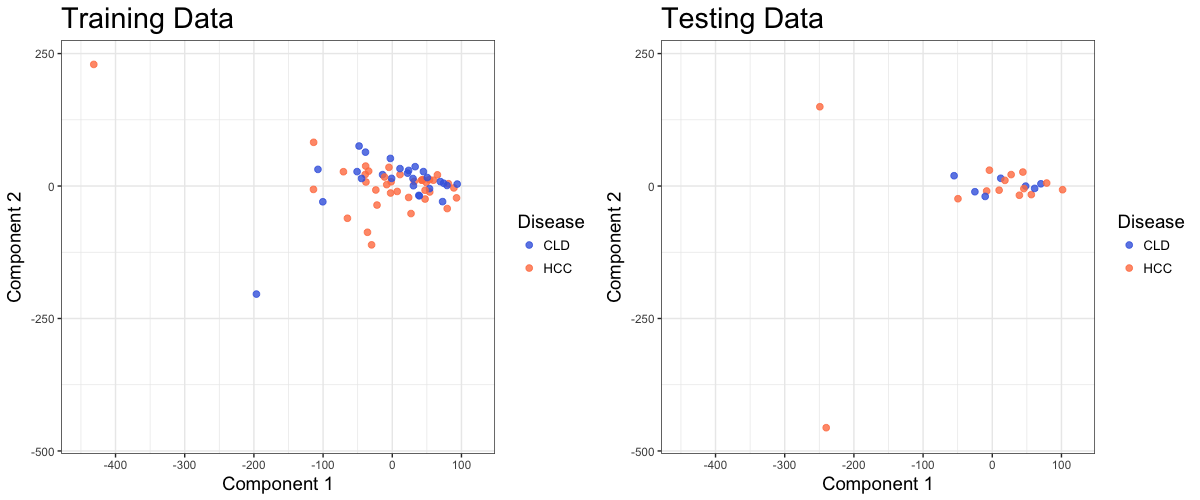
\includegraphics[scale=0.40]{Fig01.png}
\caption{PCA of Complete Data Design Matrix}
\label{fig:01}
\end{figure}

Among the patients,  $n_{1} = 51$ ($61\%$) had HCC, while the remaining $n_{0} = 33$ ($39\%$) had CLD. The complete data was randomly partitioned into training $\mathcal{D}_{\text{train}}$ and testing $\mathcal{D}_{\text{test}}$ sets containing $n_{\text{train}} = 63$ and $n_{\text{test}} = 21$ subjects, respectively. Among the training set, $n_{1,\text{train}} = 37$ ($59\%$) of patients had HCC, while among the testing set, $n_{1,\text{test}} = 14$ ($67\%$) had HCC. 

\subsection{Training Performance}
Figure (\ref{fig:02}) shows the first two principal components of the centered and scaled design matrices after features selection. Lasso achieves the best separation, followed by logistic regression and random forests, at least within the two dimensional subspace closest to the complete feature set.

\begin{figure}[h!]
\centering
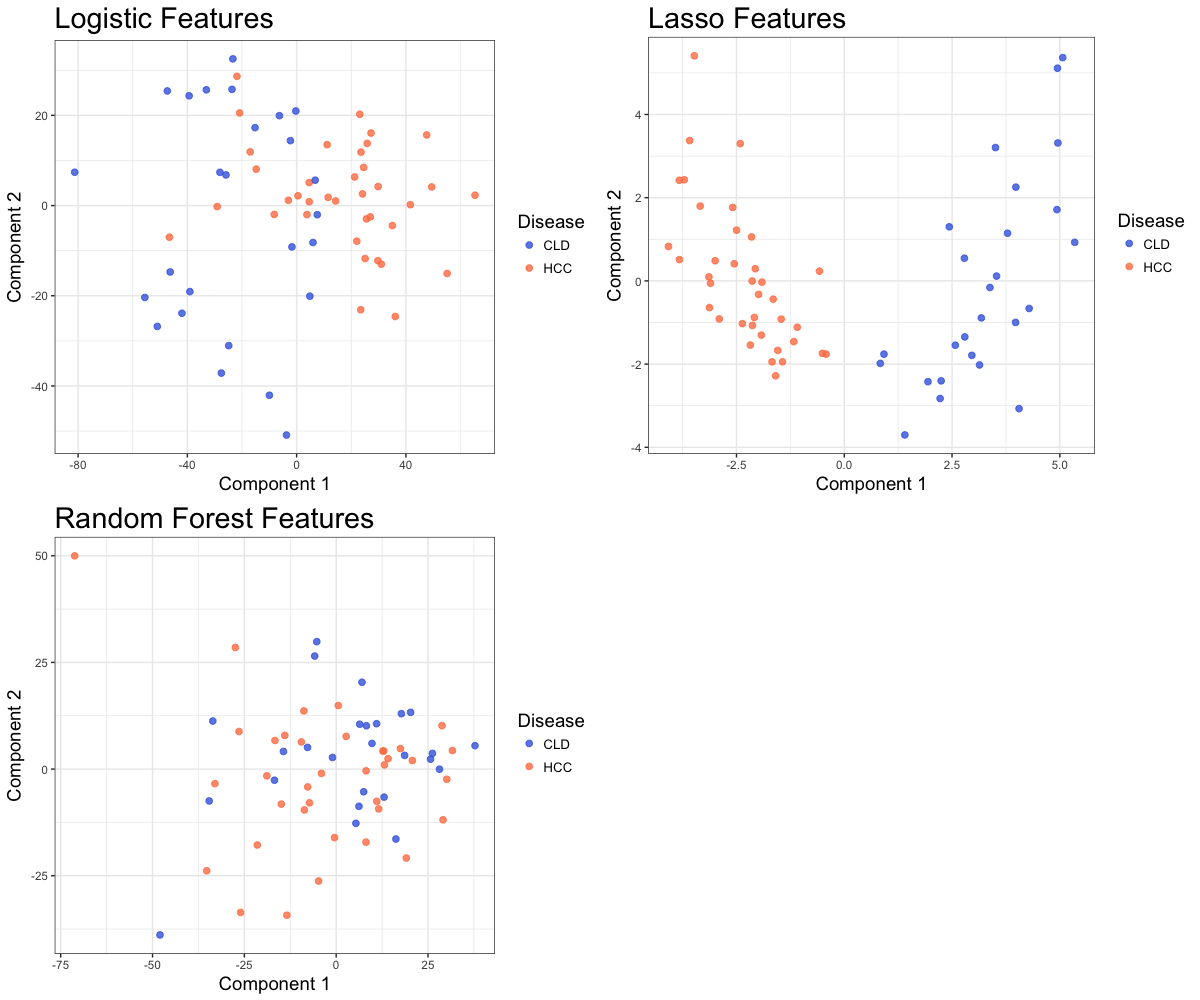
\includegraphics[scale=0.40]{Fig02.png}
\caption{PCA of Training Data Design Matrices after Feature Selection}
\label{fig:02}
\end{figure}

Figure (\ref{fig:03}) provides a heatmap of the training performance of each prediction method using features selected by lasso across the tuning parameter grid search. To increase the resolution for accuracies near one, all tuning parameter combinations achieved an accuracy less than $90\%$ are shaded white. For NNs, simple (single layer) architectures performed better than compound architectures, and a moderate learning rate was optimal. For SVMs, there was a trend towards better performance with increasing concentration. Cost exhibited a threshold effect, provided the cost was sufficiently high, little gain in performance was realized by further increases. For RFs, splitting on fewer features generally resulted in better performance than splitting on many. Among trees that split on fewer features, there was little gain in performance due to increasing the size of the forest. 

\begin{figure}[h!]
\centering
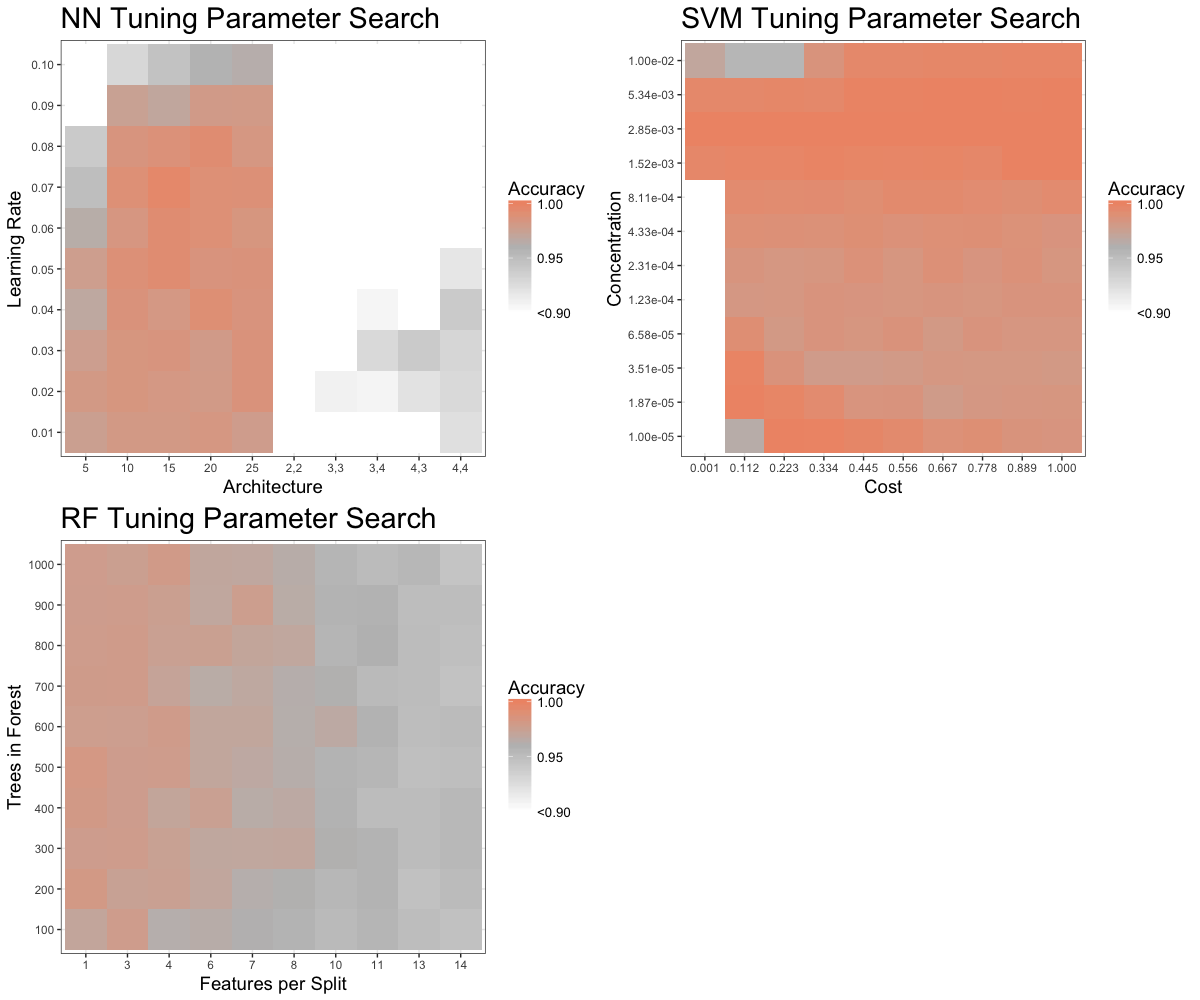
\includegraphics[scale=0.35]{Fig03.png}
\caption{Training Performance across Tuning Parameter Grid Search}
\label{fig:03}
\end{figure}


\subsubsection{Neural Networks}
Neural networks performed remarkably similarly when training on features selected by logistic regression and random forests, where each resulted in a mean accuracy of 57.9\%. Accuracy was not sensitive to the learning rate or structure of hidden layers, as shown by little variation in the classification accuracy across the 20 sets of 10-fold cross-validation. The optimal learning rate was $\eta = 0.01$ for neural networks trained on features selected by both of these methods, while the optimal structure of the hidden layers was 2 layers with 2 neurons each for logistic regression feature selection and 3 layers with 3 neurons each for feature selection by random forests. In both cases, however, the training performance was only marginally better using the best parameter values than any other combination. 

When using lasso-selected features, the training performance improved greatly when compared to the other two feature selection techniques. The mean accuracy was 88.8 \%, while the maximum was 99.5\%. Overall, neural networks with one hidden layer outperformed those with two. The accuracy was not as sensitive to the learning rate used. A single hidden layer with seven neurons and a learning rate of $\eta = 0.07$ was optimal.

\subsubsection{Support Vector Machines}
In training on features selected by marginal logistic regression, SVM achieved a mean accuracy of $75.5\%$, and maximum accuracy of $91.1\%$. Accuracy was sensitive to the choice of concentration parameter, but indifferent to the choice of cost. Optimal parameter values were $(C,\gamma) = (1,10^{-3.9})$. In training on features selected by lasso, SVM achieved a mean accuracy of $96.4\%$, and for 17 parameter combinations attained perfect accuracy. Accuracy was more sensitive to the choice of cost than of concentration. To avoid over-fitting, the parameter combination with the lowest cost was selected for the final model. Optimal parameter values were $(C,\gamma) = (10^{-3},10^{-2.6})$. In training on features selected by random forests, SVM achieved a mean accuracy of $61.0\%$, and a maximum accuracy of $67.8\%$. Accuracy was sensitive to the joint choice of concentration and cost, with some combinations performing well and others poorly. Optimal parameter values where $(C,\gamma) = (1,10^{-5})$. 

\subsubsection{Random Forests}
The random forest classifier attained maximum accuracy of 79.7  \% and average accuracy of 78.7 \%  in the training set with features selected by marginal logistic regression. The number of trees or the fraction of features chosen at each split did not make a significant difference in the accuracy; nevertheless, maximum accuracy was achieved when (\texttt{ntree}, \texttt{mtry}) = (1000,130).  In the features chosen by lasso, the random forest classifier attained maximum accuracy of 98.2 \% with parameters   (\texttt{ntree}, \texttt{mtry}) = (500,1). In this dataset the number of trees built did not improve the performance; however, as the number of features chosen at each split increased the classifier performed sub-optimally. The average accuracy was 95.1 \%. Finally, in the feature set chosen via random forest variable importance the random forest classifier had the best accuracy of 71.6 \% with (\texttt{ntree}, \texttt{mtry}) = (200,79) and the average performance was 69.9 \%.



\subsection{Testing Performance}
Table (\ref{tab:performance}) compares the training and testing performance of each prediction method trained on each feature set. 

\begin{table}[h!]
\centering
\begin{tabular}{c c | c c}
&&\multicolumn{2}{c}{Accuracy} \\
Selection & Model & Training ($\%$) & Testing ($\%$) \\ \hline
Logistic & NN & 58.7 & 66.7\\
Logistic & SVM & 91.1 & 66.7 \\
Logistic & RF & 79.7& 66.7 \\
Lasso & NN & 100 & 71.4 \\
Lasso & SVM & 100 & 66.7 \\
Lasso & RF & 98.2 & 76.2\\
RF & NN & 58.7 & 66.7\\
RF & SVM & 61.0 & 52.4 \\
RF & RF & 71.6 & 66.7\\
\end{tabular}
\caption{Comparison of Training and Testing Performance of CV-Tuned Models}
\label{tab:performance}
\end{table}

Figure (\ref{fig:04}) shows the testing performance of each prediction method optimized on each features set by 20-times repeated 10-fold cross validation. The dashed, gray line demarcates the performance of the naive classifier. Only the NN and RF classifiers trained on the features selected by Lasso outperform the naive classifier. 

\begin{figure}[h!]
\centering
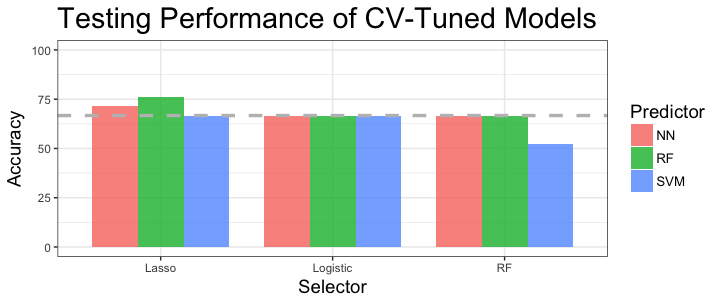
\includegraphics[scale=0.5]{Fig04.png}
\caption{Testing Performance of CV-Tuned Models}
\label{fig:04}
\end{figure}


\subsubsection{Neural Networks}
A neural network was trained for each of the three feature selection methods previously discussed using the optimal parameter values obtained via cross-validation. Each of these neural networks was then used to classify patients in the test set as either having CLD or HCC. As expected based on their training performance, the neural networks trained on features selected by logistic regression and random forests performed poorly. In fact, both classified everyone in the test set as having HCC -- the most common condition in the training set -- resulting in 66.7\% classification accuracy in the test set, where $\frac{2}{3}$ of patients had HCC. The neural network trained on lasso-selected features again performed much better, achieving an accuracy of 71.4\% in the test set. Out of seven patients with CLD, six were classified correctly (specificity = 85.7\%), while nine of fourteen HCC patients were classified correctly (sensitivity=64.3\%)

\subsubsection{Support Vector Machines}
In testing, the SVM model trained on features selected by marginal logistic regression achieved an accuracy of $67\%$. Note that this model simply predicted that all patients belonged to the most common class in the training data, i.e. HCC. All CLD patients were incorrectly classified (specificity $=0\%$), while all HCC patients were correctly classified (sensitivity $=100\%$). The SVM model trained on features selected by lasso achieved an accuracy of $67\%$. All CLD patients were correctly classified (specificity $=100\%$), however only 7 of 14 HCC patients were correctly classified (sensitivity $=50\%$). The SVM model trained on features selected by RF achieved an accuracy of $52\%$. Three of 7 CLD patients were correctly classified (specificity $=43\%$), while 8 of 14 HCC patients were correctly classified (sensitivity $=57\%$). 

\subsubsection{Random Forests}
The random forest classifiers exhibited varying accuracies across the three datasets. In both features selected by univariate logistic regression and random forest variable importance, random forest classifiers attained 66.7 \% accuracy. However, sensitivity and specificity were different between the two sets of features. When trained on features chosen by logistic regression, the random forest had sensitvity of 78.6 \% and specificity of 42.9 \%. However on the features chosen by random forest variable importance, it had sensitivity of 100\% and specificity of 0 \%, i.e. all the samples were classified as HCC. Finally, in the testing set random forest trained on lasso features had the best performance of 76.2 \%, with sensitivity of 78.6 \% and specificity of 71.4 \%. 



% Fixing the model, compare testing performance across feature sets

\section{Discussion}

\subsection{Performance of Prediction Approaches across Feature Sets}

\subsubsection{Neural Networks}
Neural networks performed quite poorly when trained on features selected by random forests or logistic regression. In fact, they both resorted to the trivial method of assigning the mode of the training set (HCC) to all patients in the test set, resulting in 0\% specificity. One possible explanation for this is that the feature sets selected by random forests and logistic regression were simply too large and contained too many non-informative transcripts. Perhaps using a stricter cutoff for the p-value and mean decrease in Gini index for logistic regression and random forests, respectively, to reduce the size of the feature sets would improve the performance of neural networks for these selection techniques. It is also possible that the parameter space searched was not large enough. 

Neural networks performed much better when paired with lasso as the feature selection technique, attaining a higher classification accuracy in the test set (71.4\%) than all others except for the random forest classifier trained on the lasso feature set. Additionally, this model had the highest specificity of all the models at 85.7\%. This increase in performance is most likely due to the fact that the feature set derived from lasso is smaller with a lower noise-to-signal ratio.

\subsubsection{Support Vector Machines}
Gaussian kernel SVMs were arguably unsuccessful as classifiers for these data, since the tuned SVM models never attained performance superior to the naive strategy of simply classifying each test patient according to the most common class in the training data. In fact the SVM model trained on features selected by logistic regression adopted this strategy, and consequently had zero specificity. The SVM model trained on features selected by lasso matched the performance of the naive classifier while retaining perfect testing specificity, but exhibited poor sensitivity. The SVM model trained on features selected by RF adopted an intermediate strategy leading to moderate sensitivity and specificity, but attained worse overall accuracy than the other models. Overall, if specificity is desirable, then the SVM trained on lasso features may have utility, however our results do not indicate that SVM is an appropriate classifier for these data. A potential explanation for the observed performance is that the Gaussian kernel is not adapted to the input data, which were integral counts prior to normalization. To test this hypothesis, we could tune SVM models using different kernels on each feature set, then evaluate performance on the testing data. Another possibility is that the Gaussian kernel is appropriate, but the tuning parameter space was not adequately explored. This explanation appears less probable because even for the SVM model trained on features selected by lasso, which performed well on the training data for all tuning parameter combinations, testing performance was unremarkable. 

\subsubsection{Random Forests}
Random forest model exhibited a notable pattern in the performance. In the training set both features selected by univariate logistic regression and random forest model didn't perform well, however the performance with the features selected through lasso had near perfect performance. One main difference between theses three sets of data is the number of features in them. Number of features selected by univariate logistic regression and random forest variable importance had thousands of features which is clearly larger than the number of samples which was 63 while the number of variables selected by lasso was 49. When there are large number of features and relatively small number of relevant features random forest classifier tend to perform poorly with small number of samples. Since only a fraction of features are selected to split the node in a tree, when there are large number of irrelevant variables the probability of a relevant variable being selected at a split is rather small. Hence using stringent cutoff for the p-value in univariate logistic regression and mean decrease in Gini index in random forest could have resulted in small number of features and in turn better performance.   

In the test set similar pattern was observed but the overall performance was not remarkable. Features selected via univariate logistic regression and random forest variable importance performed worse than the lasso feature selection. In the case of features selected via random forest variable importance the random forest classifier assigned all the samples to majority class leading to 0 \% specificity. Features selected via lasso performed marginally better than other two sets of features and sensitivity and specificity both are close to the overall performance. Yet the performance in the test set was suboptimal compared to the performance in the training set. This observation could be attributed to the fact that we had small number of training samples and random forest classifier is known to perform poorly when the training is conducted with small number of samples

\subsection{Performance of Prediction Approaches within Feature Sets}
% Fixing the feature set, compare performance of different prediction models

\subsubsection{Logistic Regression}

Our implementation of a logistic regression-based feature selection algorithm resulted in decidedly poor results for all three prediction approaches considered. All resulted in a classification accuracy of 66.7\% in the test set, which is equal to the number of HCC patients present in that set. Since the same classification accuracy could be attained by simply assigning everyone in the test set to the most prevalent condition in the training set (which is exactly what happened for both neural networks and SVM), our logistic regression feature selection provided no benefit. One likely explanation for this is that we did not use a strict enough cutoff for the p-value when deciding which features to keep. For this project, all features that obtained a p-value of less than 0.05 were kept. Because our data set originally contained 49,128 features, we would expect to keep approximately $49126 \times 0.05 \approx 2456$ on chance alone. This is a substantial portion of the $\sim 4200$ features selected using this method. Using a stricter cutoff would cut down on the number of uninformative features retained and may have resulted in better performance by all three classifiers. 

\subsubsection{Lasso}

Since lasso retains features only if the gain in model likelihood offsets the penalty on the magnitude of the regression coefficient, transcripts selected by lasso are expected to have an elevated signal to noise ratio. However, lasso cannot select more features than observations, thus the size of the training set bounds the number of candidate features retained $p \leq n$. Overall, the lasso is expected to identify a small but information dense set of transcripts. Among the models fit to the lasso features, RF achieved the best performance at $76.2\%$, followed by NN at $71.4\%$, and SVM at the baseline level of $66.7\%$. SVM had the best sensitivity at $100\%$, while NN had the best specificity at $85.7\%$. The failure of SVM to achieve better than basal accuracy on the lasso features is surprising given that most features in this set are informative. RF and NN each have an `internal' mechanism of feature  selection. If a feature is uninformative in RF, then it is unlikely to serve as splitting variable. If a feature is uninformative in NN, then its edge weights are likely to decay towards zero. In contrast, for SVM all features contribute to the estimation of similarity between observations via the kernel function, which allows noisy predictors to distort the measurement. Thus RF and NN are expected to have an advantage over SVM when the data set contains many features with a low signal to noise ratio. The improved performance of the former models on the lasso feature set suggests that RFs and NNs provide closer approximations to the true partitioning of the predictor space into decision regions. Since in SVM the kernel determines the form of decision boundaries, it is possible that the Gaussian kernel is not adapted to these data.  

\subsubsection{Random Forests}
Features selected by random forest model performed worse than other feature selection methods. Under NN and random forest classifier its performance was comparable to as if all the samples were assigned the majority label and in the case of SVM it performed worse than that. Since the cutoff for the mean decrease in Gini was determined by the top 3\% of the features in the distribution of mean decrease in Gini, a more stringent cutoff could have yielded a smaller set of features that would have been more predictive of the classes.  



\subsection{Overall Best Prediction Strategy}
% Speculate why a particular combination of feature selection and model performed best, or argue that performance among some subset of approaches was similar enough that each is expected to generalize well. 

In terms of accuracy, the RF model trained on transcripts selected by lasso provided the overall best performance, correctly classifying $76.2\%$ of the testing patients. This model consisted of an ensemble of 500 decision trees grown on bootstrap samples of the training data set. Each bifurcation in the decision trees was based on a single predictor chosen at random from the feature set. The ability to call splits based on a single, randomly selected feature likely stems from the high signal to noise ratio of transcripts in lasso feature set. Despite the ability of RF to conduct `internal' feature selection, the performance of RF was adversely affected by the presence of noisy predictors in the feature set. Evidence for this comes from comparing the testing performance of RF when trained on logistic features with performance when trained on lasso features. Forty-three of the 49 transcripts selected by lasso were contained within the feature set selected by logistic regression. Moreover, given that lasso cannot select more features than there are training observations, logistic regression was likely able to identify additional transcripts only moderately less informative than those selected by lasso. However, since feature selection by logistic regression has a type I error rate of $5\%$ and $\mathcal{O}(10^4)$ candidate transcripts were screened, it is expected that $\mathcal{O}(10^2)$ of the transcripts selected by logistic regression were false positives, i.e. associated with HCC by chance. If sufficiently many transcripts were screened at each split when training a RF on the logistic feature set, then performance comparable to a RF trained on the lasso features would be expected. Failure of the RF trained on logistic features to realize comparable performance is attributable to the presence of the false positive features. Finally, despite the demonstrated utility of RF as a prediction rule, we did not find that the variable importance metric provided by RF was useful for feature selection. In contrast to the logistic feature set, only six of the 49 transcripts selected by lasso were contained within the RF feature set. Moreover, only on the RF feature set did any model, specifically SVM, achieve performance inferior to that of the native classifier. \cite{suzuki2008dna}

\begin{figure}[h!]
\centering
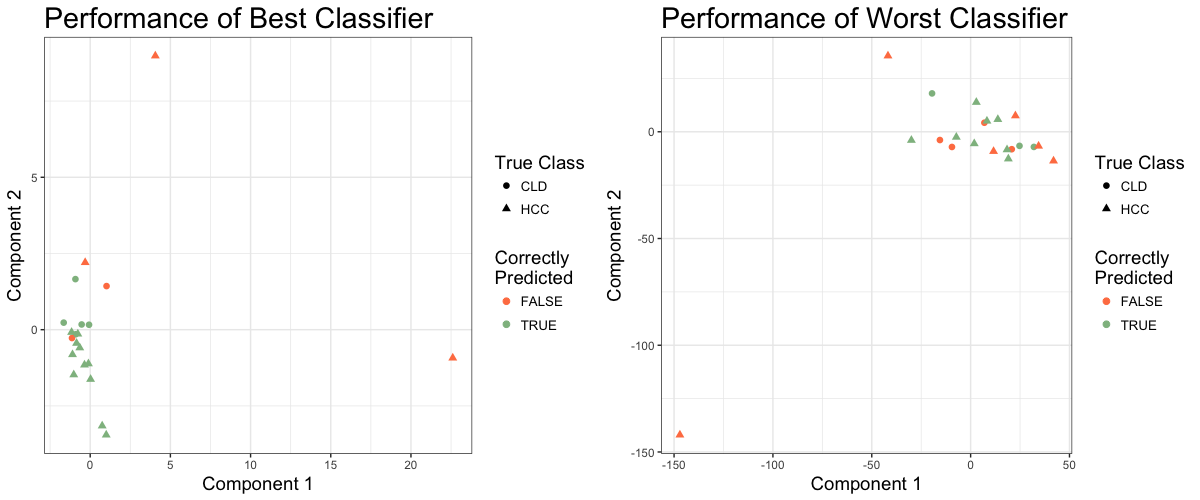
\includegraphics[scale=0.4]{Fig05.png}
\caption{Performance of Best and Worst Classifier in PC-2 Space}
\label{fig:05}
\end{figure}



%%%%%%%%%%%%%%%%%%%%%%%
	
\newpage
\bibliographystyle{plain}
\bibliography{bibfile}

%%%%%%%%%%%%%%%%%%%%%%%
\end{document}